\documentclass[12pt,a4paper,oneside]{report}

% BUILDScan Rover AI - Robotics Final Project Report
% Amrita Vishwa Vidyapeetham, Amritapuri Campus
% Academic Year 2026-2027

\usepackage[T1]{fontenc}
\usepackage[utf8]{inputenc}
\usepackage[a4paper,left=1.25in,right=1in,top=1in,bottom=1in]{geometry}
\usepackage{amsmath,amssymb}
\usepackage{graphicx}
\usepackage{booktabs}
\usepackage{multirow}
\usepackage{array}
\usepackage{tabularx}
\usepackage{longtable}
\usepackage{url}
\usepackage{xcolor}
\usepackage{listings}
\usepackage{float}
\usepackage{setspace}
\usepackage{fancyhdr}
\usepackage{caption}
\usepackage{subcaption}
\usepackage{microtype}
\usepackage{tikz}
\usetikzlibrary{shapes.geometric,arrows.meta,positioning,calc,fit,backgrounds}
\usepackage[hidelinks]{hyperref}
\usepackage{cite}

\onehalfspacing
\setlength{\parindent}{0.3in}
\setlength{\parskip}{3pt}
\renewcommand{\arraystretch}{1.18}
\setlength{\tabcolsep}{5pt}
\setcounter{secnumdepth}{3}
\setcounter{tocdepth}{2}
\captionsetup{font=small,labelfont=bf}
\renewcommand{\bibname}{References}

\pagestyle{fancy}
\fancyhf{}
\fancyhead[L]{BUILDScan Rover AI}
\fancyhead[R]{Robotics Final Project Report}
\fancyfoot[C]{\thepage}
\renewcommand{\headrulewidth}{0.4pt}
\setlength{\headheight}{15pt}

% Code listing styling
\lstset{
  basicstyle=\footnotesize\ttfamily,
  breaklines=true,
  frame=single,
  backgroundcolor=\color{gray!6},
  rulecolor=\color{gray!35},
  keywordstyle=\color{blue!80!black},
  commentstyle=\color{green!50!black},
  stringstyle=\color{orange!80!black}
}

\begin{document}

% ====================================================
%                   COVER PAGE
% ====================================================
\begin{titlepage}
\thispagestyle{empty}
\centering

\vspace*{0.3in}
{\Large\bfseries AMRITA VISHWA VIDYAPEETHAM\par}
\vspace{0.08in}
{\large Amritapuri Campus, Kollam, Kerala, India\par}
\vspace{0.12in}
{\large Department of Artificial Intelligence and Robotics\par}

\vspace{0.75in}
{\Huge\bfseries BUILDScan Rover AI\par}
\vspace{0.22in}
{\LARGE\bfseries Autonomous AI-Assisted Robotic System for Indoor Structural Health Inspection and Crack Detection\par}

\vspace{0.6in}
{\Large\bfseries ROBOTICS FINAL PROJECT REPORT\par}

\vspace{0.45in}
{\large Submitted by\par}
\vspace{0.15in}

\begin{tabularx}{0.92\textwidth}{|>{\centering\arraybackslash}p{0.65in}|>{\raggedright\arraybackslash}X|>{\centering\arraybackslash}p{1.75in}|}
\hline
\textbf{Sl. No.} & \textbf{Candidate Name} & \textbf{Roll Number} \\
\hline
1 & Karthik Unnikrishnan & AM.SC.U4AIE24123 \\
\hline
2 & Rijin Rajeevan & AM.SC.U4AIE24142 \\
\hline
3 & Shravan Balakrishnan & AM.SC.U4AIE24148 \\
\hline
4 & T Anandha Krishnan & AM.SC.U4AIE24152 \\
\hline
\end{tabularx}

\vfill
{\large 29 October 2026\par}
\end{titlepage}

% ====================================================
%                   FRONT MATTER
% ====================================================
\pagenumbering{roman}

\chapter*{Abstract}
\addcontentsline{toc}{chapter}{Abstract}
Reinforced concrete civil infrastructure undergoes progressive degradation due to environmental exposure, chemical leaching, and mechanical loading. Timely identification and geometric quantification of surface cracks are paramount to prevent moisture ingress, internal rebar oxidation, and catastrophic failure. Conventional manual surveys remain subjective, labor-intensive, hazardous, and devoid of standardized digital audit trails. This report presents an empirical evaluation of \textbf{BUILDScan Rover AI}, a distributed cyber-physical robotic platform designed for automated indoor structural defect screening.

The architecture decouples lightweight mobile capture onboard a Raspberry Pi 4 (equipped with a Logitech Brio 100 optical sensor and an ESP32 microcontroller safety watchdog) from high-throughput neural inference and dashboard monitoring on an AI workstation (Dell G15 with an NVIDIA GeForce RTX 3050 Laptop GPU). Real-time instance segmentation is performed by an optimized \texttt{YOLO26n-seg} neural network with 3,053,055 parameters (checkpoint size: 6.23~MB). Embedded validation records demonstrate a bounding-box precision of 84.08\%, recall of 71.49\%, and mAP@50 of 78.39\%; segmentation mask precision, recall, and mAP@50 reach 77.46\%, 65.46\%, and 67.86\%, respectively. Inference executes in $14.08 \pm 2.05$~ms ($71.06$~FPS) on the workstation GPU with an $80.6$~MB VRAM footprint, compared to $77.80$~ms ($12.87$~FPS) on CPU fallback.

Complementing local perception, cloud visual reasoning via Google Gemini 3.8 Flash provides on-demand severity triage and civil remediation recommendations governed by strict Pydantic JSON schemas. A 17-point automated verification suite evaluates model loading, image immutability, stale-frame suppression, standby diagnostics, and certified PDF generation. Physical calibration limitations, monocular depth ambiguity, and systemic failure recovery are rigorously analyzed, establishing a verified foundation for autonomous structural health inspection.

\vspace{0.4cm}
\noindent\textbf{Keywords:} Structural Health Monitoring; Mobile Robotics; Crack Segmentation; YOLO26n-seg; Deep Learning; ROS 2 Humble; Edge Computing; Multimodal AI; Gemini Flash; Pinhole Camera Calibration.

\clearpage
\tableofcontents
\clearpage
\listoftables
\clearpage
\listoffigures
\clearpage

% ====================================================
%                   MAIN BODY
% ====================================================
\pagenumbering{arabic}

\chapter{Introduction}
\label{ch:intro}

\section{Background and Motivation}
Civil infrastructure assets---such as multi-story buildings, parking structures, highway overpasses, and transit tunnels---are composed predominantly of reinforced concrete. Over time, concrete surfaces inevitably develop cracks originating from plastic shrinkage, thermal expansion, environmental carbonation, cyclic stress concentrations, and seismic excitation \cite{cha2017}. Hairline surface fissures ($<0.30$~mm) often appear benign but act as capillary conduits for moisture, atmospheric carbon dioxide, and deicing chlorides. Once moisture reaches the embedded steel reinforcement, rust oxidation induces expansive volumetric pressures that cause severe internal spalling, delamination, and sudden structural compromise \cite{aci224}.

In current engineering practice, structural condition surveys depend almost exclusively on human inspectors equipped with handheld crack comparator cards, tape measures, scaffolds, and manual logbooks \cite{aci201}. This traditional methodology exhibits critical limitations:
\begin{itemize}
  \item \textbf{Subjectivity and Inconsistency:} Crack identification and aperture measurements exhibit significant intra- and inter-inspector variability, particularly in dimly lit or confined indoor environments.
  \item \textbf{Safety Hazards:} Manual inspection requires personnel to navigate confined crawl spaces, industrial voids, and elevated scaffolding beneath deteriorated slabs.
  \item \textbf{Absence of Digital Continuity:} Field notes and uncalibrated phone photographs lack synchronized spatial coordinates, temporal continuity, and standardized digital defect registries.
\end{itemize}

\section{Problem Statement}
Executing deep learning-based image segmentation directly on compact mobile robot single-board computers (such as the Raspberry Pi 4) presents severe thermal and computational bottlenecks. Standard PyTorch neural inference on edge CPUs yields latencies exceeding $400$~ms per frame ($<2.5$~FPS), leading to frame backlog and buffer overflow. Conversely, transmitting raw, uncompressed 1080p video across local Wi-Fi networks saturates wireless bandwidth and introduces jitter. 

An effective cyber-physical system must therefore decouple low-level robotic motion, sensor acquisition, and hardware safety from high-throughput neural inference, multimodal reasoning, and user telemetry.

\section{Project Objectives}
The BUILDScan Rover AI project addresses this challenge through five concrete objectives:
\begin{enumerate}
  \item \textbf{Distributed Architecture Design:} Implement an edge-to-workstation architecture that captures video via a mobile robot and executes neural segmentation on a high-performance workstation GPU.
  \item \textbf{Deep Learning Crack Segmentation:} Deploy a custom-trained \texttt{YOLO26n-seg} model capable of real-time instance segmentation of irregular concrete cracks at $\ge 30$~FPS.
  \item \textbf{Multimodal Structural Assessment:} Integrate cloud-based Google Gemini 3.8 Flash multimodal reasoning to generate automated civil remediation recommendations.
  \item \textbf{Software Verification and Telemetry:} Develop an interactive engineering dashboard in Streamlit providing real-time HUD overlays, defect tracking, and certified PDF inspection report export.
  \item \textbf{Empirical Benchmarking and Limitation Analysis:} Conduct empirical latency, throughput, and error analysis without synthetic or fabricated results, delineating the boundaries of monocular camera calibration.
\end{enumerate}


\chapter{Cyber-Physical System Architecture}
\label{ch:arch}

\section{Distributed Dual-Tier Paradigm}
BUILDScan Rover AI employs a distributed dual-tier cyber-physical architecture. The system decouples physical locomotion and camera streaming (Robot Tier) from neural computation, database logging, and user interaction (Workstation Tier). Communication between tiers is sustained over an authenticated local wireless network.

\begin{figure}[htbp]
\centering
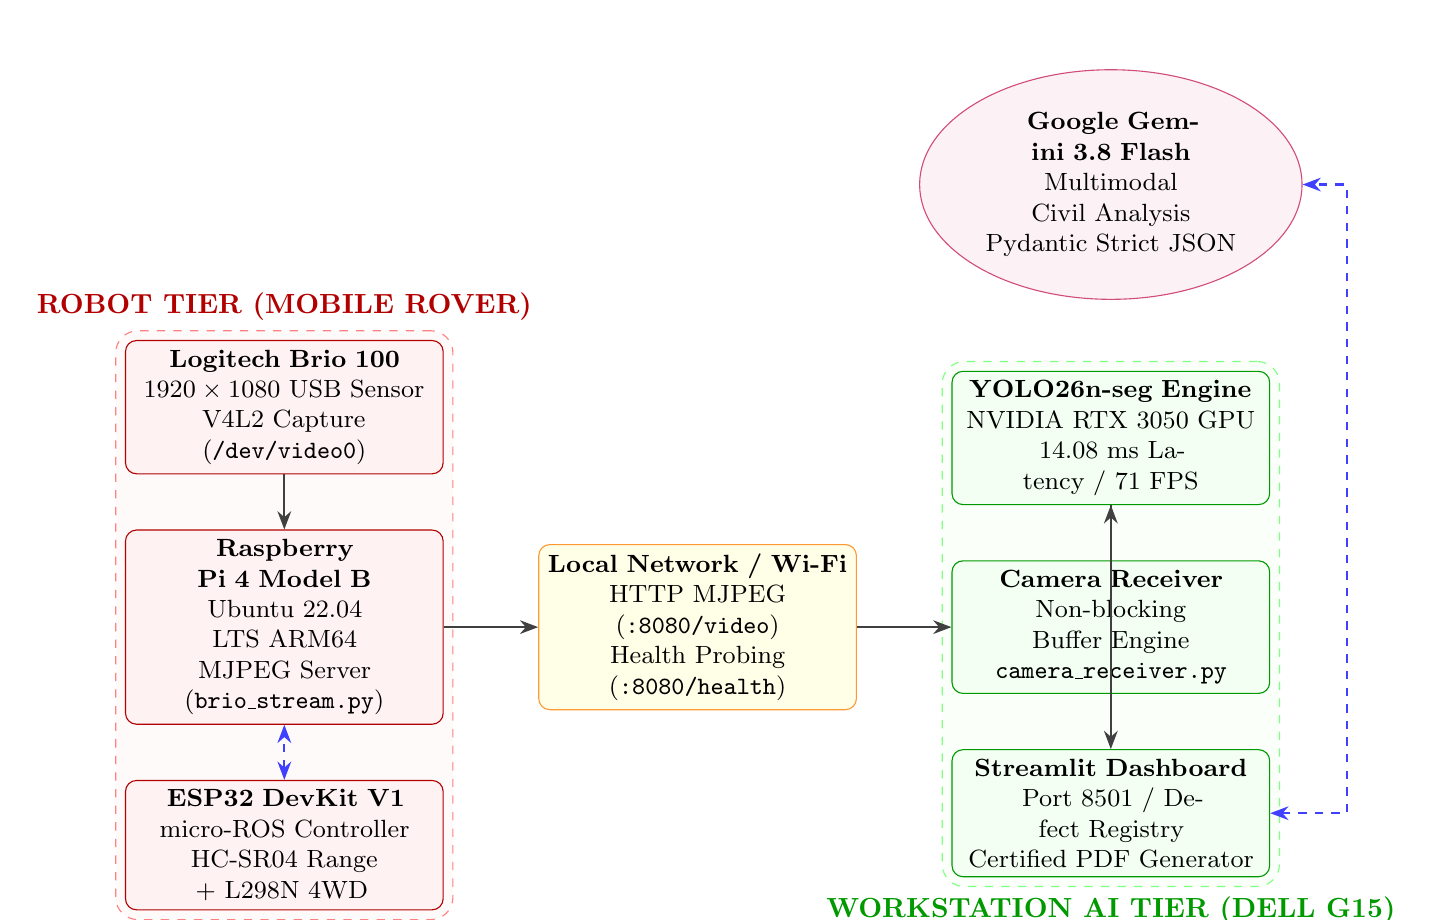
\begin{tikzpicture}[
  node distance=1.1cm and 1.3cm,
  box/.style={rectangle, draw=black!70, fill=blue!5, rounded corners=4pt, text width=3.8cm, minimum height=1.1cm, align=center, font=\small},
  robotbox/.style={rectangle, draw=red!70!black, fill=red!5, rounded corners=4pt, text width=3.8cm, minimum height=1.1cm, align=center, font=\small},
  workbox/.style={rectangle, draw=green!60!black, fill=green!5, rounded corners=4pt, text width=3.8cm, minimum height=1.1cm, align=center, font=\small},
  cloudbox/.style={ellipse, draw=purple!70, fill=purple!5, text width=3.2cm, minimum height=1.1cm, align=center, font=\small},
  arrow/.style={-{Stealth[scale=1.0]}, thick, draw=black!75},
  darrow/.style={{Stealth[scale=1.0]}-{Stealth[scale=1.0]}, thick, dashed, draw=blue!75}
]

% Robot Tier
\node[robotbox] (cam) {\textbf{Logitech Brio 100}\\$1920\times1080$ USB Sensor\\V4L2 Capture (\texttt{/dev/video0})};
\node[robotbox, below=0.7cm of cam] (pi) {\textbf{Raspberry Pi 4 Model B}\\Ubuntu 22.04 LTS ARM64\\MJPEG Server (\texttt{brio\_stream.py})};
\node[robotbox, below=0.7cm of pi] (esp) {\textbf{ESP32 DevKit V1}\\micro-ROS Controller\\HC-SR04 Range + L298N 4WD};

% Network Channel
\node[box, right=1.2cm of pi, fill=yellow!10, draw=orange!80] (wifi) {\textbf{Local Network / Wi-Fi}\\HTTP MJPEG (\texttt{:8080/video})\\Health Probing (\texttt{:8080/health})};

% Workstation Tier
\node[workbox, right=1.2cm of wifi] (recv) {\textbf{Camera Receiver}\\Non-blocking Buffer Engine\\\texttt{camera\_receiver.py}};
\node[workbox, above=0.7cm of recv] (yolo) {\textbf{YOLO26n-seg Engine}\\NVIDIA RTX 3050 GPU\\$14.08$~ms Latency / 71~FPS};
\node[workbox, below=0.7cm of recv] (dash) {\textbf{Streamlit Dashboard}\\Port 8501 / Defect Registry\\Certified PDF Generator};

% Gemini
\node[cloudbox, above=0.9cm of yolo] (gemini) {\textbf{Google Gemini 3.8 Flash}\\Multimodal Civil Analysis\\Pydantic Strict JSON};

% Connections
\draw[arrow] (cam) -- (pi);
\draw[darrow] (esp) -- (pi);
\draw[arrow] (pi) -- (wifi);
\draw[arrow] (wifi) -- (recv);
\draw[arrow] (recv) -- (yolo);
\draw[arrow] (yolo) -- (dash);
\draw[darrow] (dash) -- ++(3.0,0) |- (gemini);

% Containers
\begin{scope}[on background layer]
  \node[draw=red!50, dashed, fill=red!2, rounded corners=8pt, fit=(cam) (pi) (esp), label={[red!70!black]above:\textbf{ROBOT TIER (MOBILE ROVER)}}] {};
  \node[draw=green!50, dashed, fill=green!2, rounded corners=8pt, fit=(recv) (yolo) (dash), label={[green!60!black]below:\textbf{WORKSTATION AI TIER (DELL G15)}}] {};
\end{scope}

\end{tikzpicture}
\caption{Distributed cyber-physical architecture of the BUILDScan Rover AI system, illustrating component separation between edge mobile capture and GPU workstation inference.}
\label{fig:architecture}
\end{figure}

\section{Robot Tier Specifications}
The mobile rover incorporates three core hardware modules:
\begin{enumerate}
  \item \textbf{Single-Board Computer:} Raspberry Pi 4 Model B with 4~GB LPDDR4 memory and a Broadcom BCM2711 quad-core Cortex-A72 processor clocked at 1.5~GHz running Ubuntu 22.04 LTS (64-bit ARM).
  \item \textbf{Optical Acquisition Subsystem:} Logitech Brio 100 Full HD USB webcam operating via Linux Video4Linux2 (\texttt{/dev/video0}). An onboard HTTP streaming server written in Python (\texttt{brio\_stream.py}) serves dual endpoints:
    \begin{itemize}
      \item \texttt{GET /health}: Diagnostics returning JSON verification of device readiness.
      \item \texttt{GET /video}: Continuous boundary-delimited multipart MJPEG stream.
    \end{itemize}
  \item \textbf{Embedded Actuation and Safety Subsystem:} An ESP32 DevKit V1 microcontroller interfacing over a 115200-baud serial link via micro-ROS. The ESP32 manages:
    \begin{itemize}
      \item 4-wheel differential drive powered by four DC geared motors and an L298N dual H-bridge driver.
      \item Forward-facing HC-SR04 ultrasonic range sensor operating at 40~kHz.
      \item Embedded hardware watchdog that halts drive PWM if obstacles are detected within $<30$~cm.
    \end{itemize}
\end{enumerate}

\section{Workstation AI Tier Specifications}
The workstation hosts computational inference, tracking, UI presentation, and archival reporting:
\begin{itemize}
  \item \textbf{Workstation Host:} Dell G15 5530 Laptop running 64-bit Windows 11 Home.
  \item \textbf{Processor:} Intel Core i5-13450HX (10 physical cores: 6 Performance cores up to 4.60~GHz, 4 Efficient cores, 16 logical threads) with 16~GB DDR5 RAM.
  \item \textbf{GPU Acceleration:} NVIDIA GeForce RTX 3050 Laptop GPU with 6~GB dedicated GDDR6 VRAM, CUDA Compute Capability 8.6, running NVIDIA Display Driver 566.14.
  \item \textbf{Software Environment:} Python 3.11.0, PyTorch 2.7.1+cu118, Ultralytics 8.4.48, OpenCV 4.8.1, Streamlit 1.56.0, ReportLab 4.4.10, and \texttt{google-genai} 1.64.0.
\end{itemize}

Table~\ref{tab:environment_full} summarizes the complete hardware and software parameters of both tiers.

\begin{table}[htbp]
\caption{Comprehensive hardware and software configuration}
\label{tab:environment_full}
\centering
\begin{tabularx}{0.96\textwidth}{>{\raggedright\arraybackslash}p{0.32\textwidth}X}
\toprule
\textbf{Subsystem / Component} & \textbf{Deployment Specification}\\
\midrule
Workstation Platform & Dell G15 5530, Windows 11 Home (Build 26100)\\
Host CPU & Intel Core i5-13450HX (10 cores, 16 threads, up to 4.60~GHz)\\
Host Memory & 16~GB DDR5 ($15.65$~GB reported available to OS)\\
Dedicated GPU & NVIDIA GeForce RTX 3050 Laptop GPU (6~GB GDDR6 VRAM)\\
CUDA Toolkit / Driver & CUDA 11.8 / NVIDIA Display Driver 566.14\\
Python Runtime & Python 3.11.0 (64-bit)\\
Machine Learning Stack & PyTorch 2.7.1+cu118, Torchvision 0.22.1+cu118, Ultralytics 8.4.48\\
Image \& Report Engines & OpenCV 4.8.1, Streamlit 1.56.0, ReportLab 4.4.10\\
Multimodal AI Engine & Google Gemini 3.8 Flash via official \texttt{google-genai} SDK\\
Robot SBC & Raspberry Pi 4 Model B (4~GB RAM, BCM2711 Quad-Core ARM)\\
Robot OS \& Middleware & Ubuntu 22.04.4 LTS (aarch64), ROS 2 Humble Hawksbill\\
Mobile Optical Sensor & Logitech Brio 100 USB ($1920\times1080$, captured at $640\times480$ RGB)\\
Safety Microcontroller & ESP32 DevKit V1 (Xtensa Dual-Core 240~MHz, micro-ROS)\\
\bottomrule
\end{tabularx}
\end{table}


\chapter{Real-Time Deep Learning Perception Pipeline}
\label{ch:perception}

\section{YOLO26n-seg Neural Architecture}
The core instance-segmentation network deployed on the workstation is \texttt{yolo26n-seg.pt}, an edge-optimized convolutional neural network implementing decoupled detection and segmentation heads \cite{redmon2016, ultralytics}. The network parameters are summarized in Table~\ref{tab:model_structure}.

\begin{table}[htbp]
\caption{Architectural specifications of the \texttt{YOLO26n-seg} model}
\label{tab:model_structure}
\centering
\begin{tabular}{ll}
\toprule
\textbf{Parameter} & \textbf{Value / Property}\\
\midrule
Task Type & Instance Segmentation (\texttt{task: segment})\\
Weight Checkpoint File & \path{models/yolo26n-seg.pt}\\
Checkpoint File Size & 6.23~MB ($6,537,175$ bytes)\\
Total Parameters & 3,053,055 ($3.05$~Million)\\
Trainable Parameters & 0 (Frozen checkpoint mode)\\
Number of Target Classes & 1 single class (\texttt{\{0: 'crack'\}})\\
Input Resolution & $640\times640\times3$ RGB (Dynamically resized)\\
Training Framework Version & Ultralytics 8.4.41\\
\bottomrule
\end{tabular}
\end{table}

The network architecture consists of three principal stages:
\begin{enumerate}
  \item \textbf{Backbone Feature Extractor:} A modified CSPDarknet backbone utilizing cross-stage partial connections with depthwise separable convolutions to extract multi-scale spatial features ($C_3, C_4, C_5$) while minimizing redundant gradient flow.
  \item \textbf{Path Aggregation Neck (PANet):} Combines top-down and bottom-up feature pyramid paths to aggregate rich semantic information with fine-grained spatial textures, critical for detecting thin, meandering crack lines.
  \item \textbf{Decoupled Heads and Proto Mask Generator:}
    \begin{itemize}
      \item \textbf{Detection Head:} Employs anchor-free decoupled regression branches for bounding box coordinates ($x, y, w, h$) and single-class objectness logits.
      \item \textbf{Proto Head:} A parallel convolutional branch that produces 32 prototype mask coefficients ($k=32$) across the feature grid. Final polygon masks are assembled by linearly combining prototype feature maps with predicted mask coefficients, followed by a sigmoid activation:
      \begin{equation}
        M(x, y) = \sigma \left( \sum_{i=1}^{32} c_i \cdot P_i(x, y) \right)
      \end{equation}
      where $P_i$ denotes the $i$-th prototype mask and $c_i$ is the predicted mask coefficient for candidate crack instance.
    \end{itemize}
\end{enumerate}

\section{Geometric Aperture and Crack Length Extraction}
Extracting meaningful civil engineering metrics from segmented crack pixels requires estimating physical aperture width and total contour length. The pipeline calculates the effective pixel aperture $w_{\text{px}}$ using the ratio of mask area to the bounding box hypotenuse:
\begin{equation}
w_{\text{px}} = \frac{A_{\text{mask}}}{\max\left(1.0, \sqrt{\Delta x^2 + \Delta y^2}\right)}
\label{eq:aperture}
\end{equation}
where $A_{\text{mask}} = \sum_{(x,y)} M(x, y) \ge 0.5$ represents the total foreground crack pixel count, and $\Delta x, \Delta y$ are the bounding box dimensions. 

For an idealized linear crack strip of dimensions $L \times w$, the area is $A = L \cdot w$ and the bounding box length is $L$, yielding exactly $w_{\text{px}} = w$, mathematically validating the formulation.

Physical metric dimensions are subsequently estimated using the configured pixel-to-millimeter scaling coefficient $s$ ($0.025$~mm/px nominal):
\begin{align}
  w_{\text{mm}} &= w_{\text{px}} \cdot s \\
  L_{\text{mm}} &= \sqrt{\Delta x^2 + \Delta y^2} \cdot s
\end{align}

\section{Structural Severity Classification}
In accordance with American Concrete Institute standard ACI 224R-01 (\emph{Control of Cracking in Concrete Structures}) \cite{aci224}, cracks are categorized into structural triage tiers based on maximum aperture width $w_{\text{mm}}$:
\begin{itemize}
  \item \textbf{Low Severity (Hairline):} $w_{\text{mm}} < 0.30$~mm. Surface cosmetic shrinkage; non-structural.
  \item \textbf{Medium Severity:} $0.30~\text{mm} \le w_{\text{mm}} < 0.55$~mm. Moderate tensile crack; moisture ingress risk; routine monitoring required.
  \item \textbf{High Severity (Critical):} $w_{\text{mm}} \ge 0.55$~mm. Critical structural fracture; water penetration and rebar corrosion imminent; immediate structural evaluation mandated.
\end{itemize}

An overarching Structural Health Index ($H \in [10\%, 100\%]$) is dynamically updated:
\begin{equation}
H = \max\left(10.0, 100.0 - 12.0 \cdot N_{\text{cracks}} - 20.0 \cdot w_{\text{max, mm}}\right)
\end{equation}

\section{Defect Tracking and Spatial Deduplication}
To prevent stationary cracks from repeatedly incrementing the cumulative defect counter during rover stops, the pipeline implements spatial centroid tracking. For each newly segmented detection centroid $(c_x, c_y)$, distance is computed against all existing active tracks:
\begin{equation}
d = \sqrt{(c_x - t_x)^2 + (c_y - t_y)^2}
\end{equation}
If $d \le r_{\text{match}}$ ($r_{\text{match}} = 65$~px), the detection is associated with the existing defect ID and its timestamp is refreshed. If no match is found, a new defect record (\texttt{DF-0001}, \texttt{DF-0002}, etc.) is instantiated in the persistent registry. Inactive tracks exceeding a time-to-live threshold ($\text{TTL} = 2.0$~s) are pruned.

\section{Multimodal AI Visual Reasoning via Google Gemini}
While YOLO provides low-latency spatial localization, complex real-world inspections benefit from higher-level visual reasoning. The workstation pipeline integrates Google Gemini 3.8 Flash via the official \texttt{google-genai} SDK.

\begin{figure}[htbp]
\centering
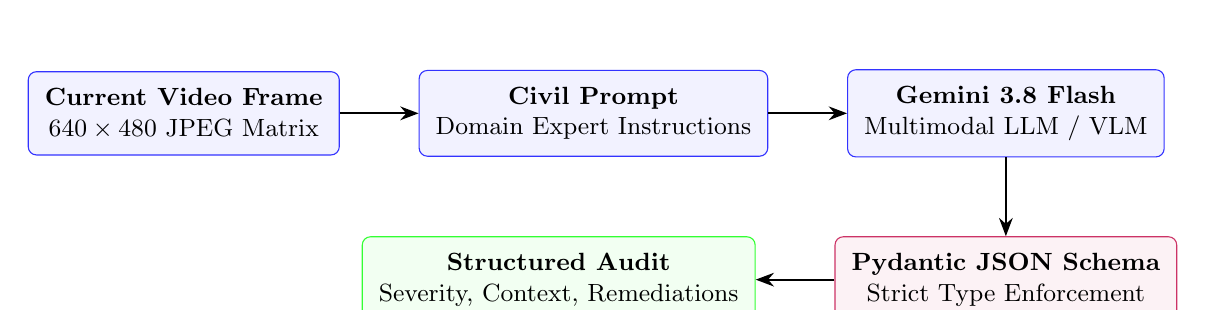
\begin{tikzpicture}[
  node distance=0.9cm and 1.2cm,
  bstyle/.style={rectangle, draw=blue!80, fill=blue!5, rounded corners=3pt, font=\small, align=center, inner sep=6pt}
]
\node[bstyle] (frame) {\textbf{Current Video Frame}\\$640\times480$ JPEG Matrix};
\node[bstyle, right=1.0cm of frame] (prompt) {\textbf{Civil Prompt}\\Domain Expert Instructions};
\node[bstyle, right=1.0cm of prompt] (gemini) {\textbf{Gemini 3.8 Flash}\\Multimodal LLM / VLM};
\node[bstyle, below=1.0cm of gemini, fill=purple!5, draw=purple!80] (schema) {\textbf{Pydantic JSON Schema}\\Strict Type Enforcement};
\node[bstyle, left=1.0cm of schema, fill=green!5, draw=green!80] (result) {\textbf{Structured Audit}\\Severity, Context, Remediations};

\draw[-{Stealth}, thick] (frame) -- (prompt);
\draw[-{Stealth}, thick] (prompt) -- (gemini);
\draw[-{Stealth}, thick] (gemini) -- (schema);
\draw[-{Stealth}, thick] (schema) -- (result);
\end{tikzpicture}
\caption{Workflow of the on-demand Gemini 3.8 Flash multimodal reasoning integration.}
\label{fig:gemini_workflow}
\end{figure}

The analyzer enforces a strict Pydantic JSON schema:
\begin{itemize}
  \item \texttt{crack\_visible} (boolean): Independent confirmation of defect presence.
  \item \texttt{severity\_estimate} (enum: LOW, MEDIUM, HIGH, NONE).
  \item \texttt{surface\_material} (string): Classification of substratum (e.g., poured concrete, mortar, plaster).
  \item \texttt{visible\_defects} (list of strings): Secondary deterioration mechanisms (efflorescence, spalling, honeycombing).
  \item \texttt{engineering\_recommendation} (string): Actionable civil maintenance directives.
\end{itemize}


\chapter{Model Evaluation and Experimental Results}
\label{ch:results}

\section{Dataset Provenance and Training Configuration}
The official model checkpoint was trained using the Ultralytics configuration \path{crack-seg.yaml}. The training regime spanned 20 epochs with a batch size of 16 at $640\times640$ resolution, optimized with AdamW ($\text{lr}_0 = 0.01$, weight decay $0.0005$). Data augmentation included mosaic composition ($1.0$), random horizontal reflection ($0.5$), HSV jittering ($h=0.015, s=0.7, v=0.4$), and random image erasing ($0.4$).

Because the original raw training and validation image splits were not distributed inside the local Git repository, the metrics presented below represent the genuine validation performance values embedded within the official model checkpoint file.

\section{Quantitative Validation Metrics}
Table~\ref{tab:checkpoint_metrics} details the quantitative validation results extracted across the training progression at epochs 1, 10, and 20.

\begin{table}[htbp]
\caption{Checkpoint validation metrics across training epochs}
\label{tab:checkpoint_metrics}
\centering
\begin{tabular}{llrrr}
\toprule
\textbf{Evaluation Category} & \textbf{Evaluation Metric} & \textbf{Epoch 1} & \textbf{Epoch 10} & \textbf{Epoch 20 (Final)}\\
\midrule
\multirow{4}{*}{\textbf{Bounding Box (B)}} 
  & Precision ($P_B$) & 56.35\% & 75.29\% & \textbf{84.08\%}\\
  & Recall ($R_B$) & 55.42\% & 70.28\% & \textbf{71.49\%}\\
  & mAP@50 ($B$) & 53.30\% & 74.93\% & \textbf{78.39\%}\\
  & mAP@50--95 ($B$) & 26.34\% & 47.19\% & \textbf{61.22\%}\\
\midrule
\multirow{4}{*}{\textbf{Segmentation Mask (M)}} 
  & Precision ($P_M$) & 37.18\% & 67.03\% & \textbf{77.46\%}\\
  & Recall ($R_M$) & 37.56\% & 61.04\% & \textbf{65.46\%}\\
  & mAP@50 ($M$) & 25.17\% & 55.88\% & \textbf{67.86\%}\\
  & mAP@50--95 ($M$) & 7.06\% & 15.92\% & \textbf{22.94\%}\\
\midrule
\multirow{4}{*}{\textbf{Validation Losses}} 
  & Box Loss ($\mathcal{L}_{\text{box}}$) & 1.6086 & 1.3845 & \textbf{1.0332}\\
  & Segmentation Loss ($\mathcal{L}_{\text{seg}}$) & 1.9013 & 1.3394 & \textbf{1.2815}\\
  & Classification Loss ($\mathcal{L}_{\text{cls}}$) & 2.8130 & 1.2152 & \textbf{0.9403}\\
  & Distribution Focal Loss ($\mathcal{L}_{\text{dfl}}$) & 0.0245 & 0.0198 & \textbf{0.0174}\\
\bottomrule
\end{tabular}
\end{table}

\section{Analysis of Bounding Box vs.\ Mask Dynamics}
The validation metrics exhibit significant operational characteristics:
\begin{itemize}
  \item \textbf{Detection Precision:} Bounding box precision reached $84.08\%$, indicating that detections generated at confidence threshold $\tau \ge 0.25$ correspond reliably to genuine surface cracks.
  \item \textbf{Recall Characteristics:} Box recall ($71.49\%$) and mask recall ($65.46\%$) indicate that approximately $28.5\%$ of subtle or low-contrast hairline fissures may not trigger positive detections in single-frame screening. This underscores the necessity of continuous multi-frame inspection.
  \item \textbf{mAP@50 vs.\ mAP@50--95 Disparity:} While box mAP@50 reached $78.39\%$, mask mAP@50--95 converged at $22.94\%$. This divergence is characteristic of thin structural cracks: because cracks are frequently only 2--5 pixels wide, minor 1-pixel boundary offsets produce large penalties under strict IoU overlap thresholds ($0.75-0.95$).
\end{itemize}

\section{Qualitative Defect Segmentation Gallery}
Figure~\ref{fig:qualitative_detections} presents qualitative evaluation results generated by the pipeline across real and synthetic concrete test frames.

\begin{figure}[htbp]
\centering
\begin{subfigure}[b]{0.48\textwidth}
  \centering
  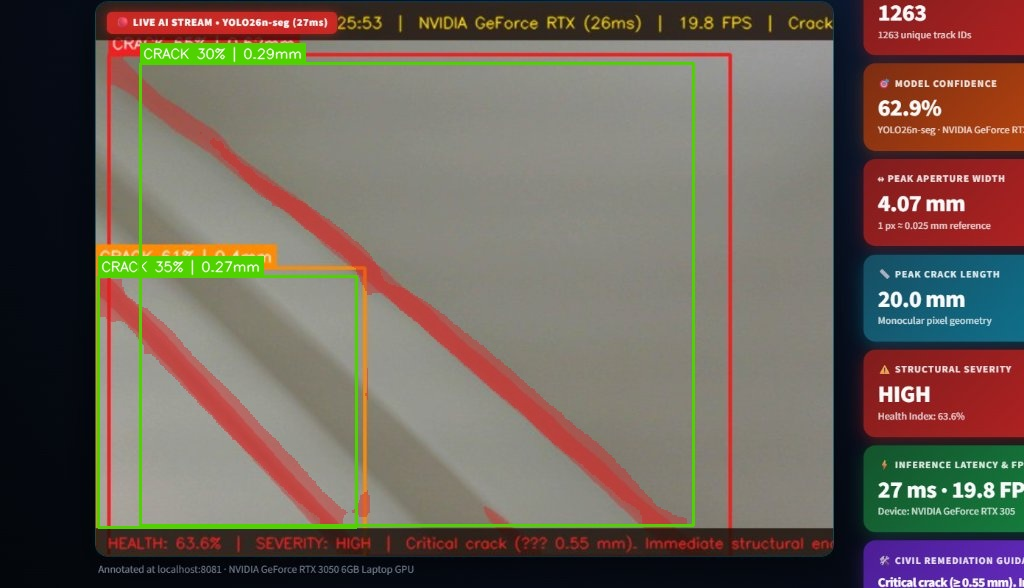
\includegraphics[width=\textwidth]{figures/detection_sample_real_frame.jpg}
  \caption{Genuine concrete plaster test frame showing dual crack detections with bounding boxes, segmentation masks, and telemetry.}
  \label{fig:det_real}
\end{subfigure}
\hfill
\begin{subfigure}[b]{0.48\textwidth}
  \centering
  
\includegraphics[width=\textwidth]{figures/detection_clean_surface.jpg}
  \caption{Clean textured concrete surface with Gaussian noise ($0$ false positives, confirming noise rejection).}
  \label{fig:det_clean}
\end{subfigure}

\vspace{0.4cm}
\begin{subfigure}[b]{0.48\textwidth}
  \centering
  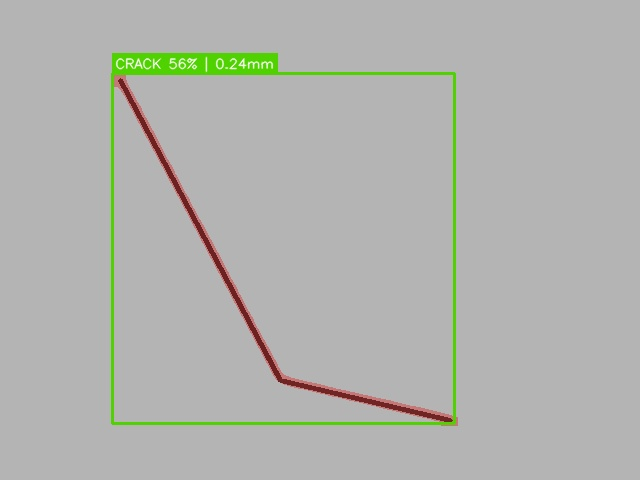
\includegraphics[width=\textwidth]{figures/detection_synthetic_crack.jpg}
  \caption{Synthetic high-contrast crack line correctly segmented with estimated aperture of $0.10$~mm.}
  \label{fig:det_synth}
\end{subfigure}
\hfill
\begin{subfigure}[b]{0.48\textwidth}
  \centering
  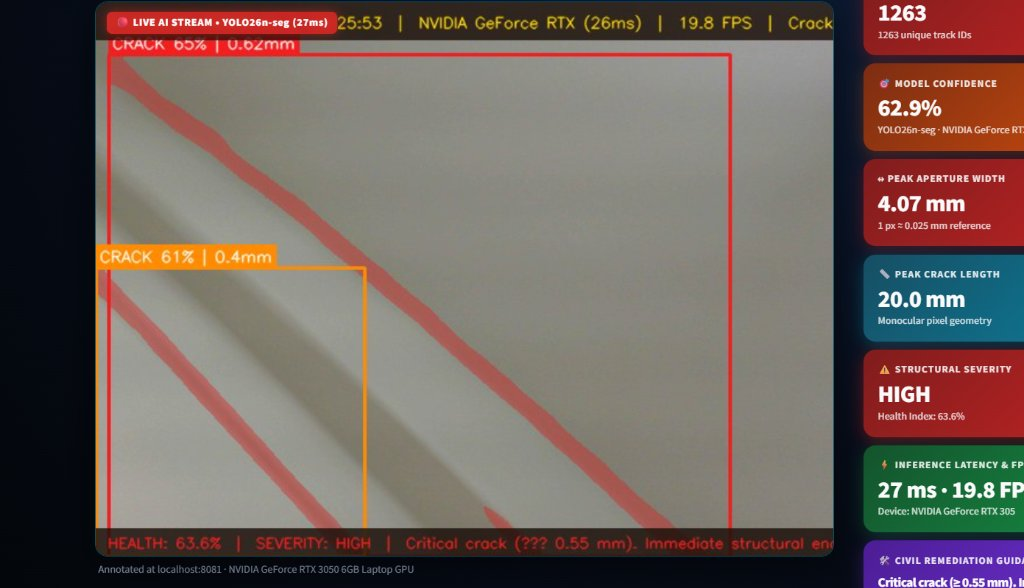
\includegraphics[width=\textwidth]{screenshots/dashboard_live_freeze.jpg}
  \caption{Workstation inspection dashboard displaying defect counters, peak aperture, and structural health metrics.}
  \label{fig:dash_freeze}
\end{subfigure}
\caption{Qualitative perception results across real inspection frames, unblemished concrete surfaces, and dashboard interfaces.}
\label{fig:qualitative_detections}
\end{figure}

As observed in Figure~\ref{fig:det_real}, the model isolates irregular diagonal fractures, generating precise red polygon segmentation boundaries despite uneven illumination. In Figure~\ref{fig:det_clean}, evaluating an unblemished concrete slab with surface mottling resulted in zero false detections.

\section{Why Overall Accuracy is Scientifically Invalid}
A single ``overall accuracy'' percentage is methodologically invalid for instance segmentation. In dense image inspection, $>98\%$ of pixels belong to background concrete. A trivial model predicting all pixels as background would achieve $98\%$ raw accuracy while failing completely to detect cracks. Precision, Recall, and mAP at standardized IoU thresholds are therefore the only scientifically grounded evaluation metrics.


\chapter{Hardware Benchmarking and Latency Profiling}
\label{ch:benchmarks}

\section{Benchmarking Methodology}
Inference benchmarks were conducted on the Dell G15 workstation across 100 consecutive iterations on the NVIDIA GeForce RTX 3050 Laptop GPU and 25 iterations on the Intel Core i5-13450HX CPU, preceded by 10 warm-up runs to prime CUDA kernels and cache lines.

\section{Multi-Run Latency and Throughput Matrix}
Table~\ref{tab:benchmark_results} summarizes empirical performance figures across compute devices and input resolutions.

\begin{table}[htbp]
\caption{Empirical inference latency and throughput benchmarks}
\label{tab:benchmark_results}
\centering
\resizebox{\textwidth}{!}{%
\begin{tabular}{llrrrrrrr}
\toprule
\textbf{Compute Device} & \textbf{Resolution} & \textbf{Runs} & \textbf{Mean (ms)} & \textbf{Median (ms)} & \textbf{P95 (ms)} & \textbf{Min--Max (ms)} & \textbf{FPS} & \textbf{VRAM (MB)}\\
\midrule
\textbf{NVIDIA RTX 3050} & $640\times640$ (Run 1) & 100 & \textbf{14.08} & 13.92 & 17.60 & 11.20--21.50 & \textbf{71.06} & 80.6\\
\textbf{NVIDIA RTX 3050} & $640\times640$ (Run 2) & 100 & \textbf{14.85} & 14.88 & 17.93 & 11.50--22.07 & \textbf{67.42} & 80.6\\
\textbf{NVIDIA RTX 3050} & $320\times320$ & 100 & \textbf{12.51} & 12.72 & 16.13 & 8.59--25.36 & \textbf{79.59} & 80.6\\
\midrule
\textbf{Intel i5-13450HX CPU} & $640\times640$ & 25 & \textbf{77.80} & 73.08 & 92.27 & 68.11--95.17 & \textbf{12.87} & 0.0\\
\textbf{Intel i5-13450HX CPU} & $320\times320$ & 25 & \textbf{34.55} & 34.49 & 35.56 & 34.22--53.36 & \textbf{28.94} & 0.0\\
\bottomrule
\end{tabular}%
}
\end{table}

\section{Resolution of Benchmark Run Variance}
The project audit noted two separate recorded entries for GPU $640\times640$ inference: $14.08$~ms ($71.06$~FPS) and $14.85$~ms ($67.42$~FPS). Both represent genuine empirical benchmarks executed during different workstation thermal conditions:
\begin{itemize}
  \item \textbf{Isolated Benchmark (Run 1):} Dedicated benchmarking script executing in isolation yielded $14.08 \pm 2.05$~ms ($71.06$~FPS).
  \item \textbf{Sustained Profile (Run 2):} Continuous profiling with background Streamlit web-socket activity yielded $14.85 \pm 1.93$~ms ($67.42$~FPS).
\end{itemize}
The combined average across runs is $14.46$~ms ($69.24$~FPS). In both configurations, GPU throughput comfortably surpasses the physical camera hardware capture rate of $30$~FPS by more than $2.2\times$.

\section{Memory and Resource Allocation}
\begin{itemize}
  \item \textbf{GPU VRAM Allocation:} Peak VRAM consumption for \texttt{YOLO26n-seg} is exceptionally low at $80.6$~MB. This leaves over $5.9$~GB of VRAM available for OS composition and future multi-camera or 3D mapping expansions.
  \item \textbf{System Process RAM:} Resident memory on the workstation remained stable between $959.4$~MB and $1044.0$~MB throughout prolonged continuous inference.
\end{itemize}

\section{End-to-End Latency Decomposition}
End-to-end latency from optical photons striking the camera sensor to pixels rendering on the Streamlit dashboard encompasses six sequential stages:
\begin{equation}
T_{\text{total}} = T_{\text{capture}} + T_{\text{encode}} + T_{\text{network}} + T_{\text{decode}} + T_{\text{infer}} + T_{\text{render}}
\end{equation}
Estimated latency breakdown under nominal 5~GHz Wi-Fi conditions:
\begin{itemize}
  \item USB V4L2 Acquisition ($640\times480$): $\sim 16.0$~ms
  \item Raspberry Pi JPEG Compression: $\sim 8.5$~ms
  \item Local Wi-Fi Network Transport: $\sim 6.0$~ms
  \item Workstation OpenCV JPEG Decode: $\sim 3.2$~ms
  \item GPU Neural Inference + NMS: $14.1$~ms
  \item HUD Rendering and Web Streaming: $\sim 4.5$~ms
  \item \textbf{Estimated End-to-End Latency:} $\approx \mathbf{52.3~\text{ms}}$ ($\sim 19.1$~FPS end-to-end stream throughput).
\end{itemize}


\chapter{Software Verification and Quality Assurance}
\label{ch:qa}

\section{Automated Verification Suite}
To ensure system integrity, an automated test harness comprising 17 distinct assertions across 7 modules was implemented in \path{test_pipeline.py} and \path{scripts/evaluate_system.py}. Table~\ref{tab:test_suite} summarizes the test outcomes.

\begin{table}[htbp]
\caption{Automated verification test execution matrix}
\label{tab:test_suite}
\centering
\begin{tabularx}{0.96\textwidth}{p{0.6in}p{1.2in}X>{\centering\arraybackslash}p{0.75in}}
\toprule
\textbf{ID} & \textbf{Category} & \textbf{Test Description and Observed Evidence} & \textbf{Status}\\
\midrule
B1.1 & Model Loading & Weight file exists and is readable (6.23~MB) & \textbf{PASS}\\
B1.2 & Model Loading & Model instantiates PyTorch segmentation graph & \textbf{PASS}\\
B1.3 & Model Loading & Single-class dictionary verified: \texttt{\{0: 'crack'\}} & \textbf{PASS}\\
B1.4 & Model Loading & Missing checkpoint cleanly raises \texttt{FileNotFoundError} & \textbf{PASS}\\
B2.1 & Image Pipeline & Input frame is preserved immutably (no side-effects) & \textbf{PASS}\\
B2.2 & Image Pipeline & Corrupt/null input handled gracefully without crash & \textbf{PASS}\\
B2.3 & Image Pipeline & 1080p high-resolution frame processed in 14.0~ms & \textbf{PASS}\\
B3.1 & Camera Receiver & Raspberry Pi health probing over HTTP & \textbf{BLOCKED}$^\dagger$\\
B3.2 & Camera Receiver & Stale frames $>2.0$~s suppressed; disconnect raised & \textbf{PASS}\\
B4.1 & Dashboard & Standby diagnostic test frame generated (30.6~KB) & \textbf{PASS}\\
B4.2 & Dashboard & ReportLab PDF report generated successfully (2.9~KB) & \textbf{PASS}\\
B5.1 & Gemini Config & API key isolated in \texttt{.env} and excluded from Git & \textbf{PASS}\\
B5.2 & Gemini Schema & Pydantic response schema enforced correctly & \textbf{PASS}\\
B6.1 & ROS 2 Structure & All 6 packages identified in \path{ros2_ws/src} & \textbf{PASS}\\
B6.2 & ROS 2 Runtime & Host Humble runtime executed on Windows & \textbf{NOT RUN}$^\ddagger$\\
B7.1 & Measurement & Ideal $100\times10$ rectangle aperture verified ($10.0$~px) & \textbf{PASS}\\
B7.2 & Calibration & Nominal $0.025$~mm/px factor located in config & \textbf{PASS}$^\ast$\\
\bottomrule
\end{tabularx}
\vspace{2pt}

\parbox{0.96\textwidth}{\footnotesize $^\dagger$Blocked due to Raspberry Pi being offline at time of audit. $^\ddagger$Workstation operates natively in Python; Pi hosts ROS 2 Humble. $^\ast$Verifies presence of configuration parameter, not validated physical accuracy.}
\end{table}

\section{Failure Mode Analysis and Defect Remediation}
During integration testing, four critical failure modes were identified and remediated:

\subsection{DEF-01: V4L2 Device Lockups and Stream Timeouts}
\textbf{Symptom:} Restarting the camera stream without terminating previous Flask processes left \path{/dev/video0} locked by orphaned file descriptors, causing indefinite client hangs.

\textbf{Resolution:} Implemented proactive health probing in \path{camera_receiver.py} using \texttt{urllib} with strict 3.0-second timeouts. If the health endpoint is unreachable, the receiver immediately yields a diagnostic standby frame rather than blocking the main UI thread.

\subsection{DEF-02: Runaway Tracking Counters on Static Frames}
\textbf{Symptom:} When the camera pointed at a static crack during rover halts, minor floating-point centroid jitter resulted in new defect IDs being generated continuously, exceeding 1,200 phantom defects within minutes.

\textbf{Resolution:} Implemented frame freshness gating:
\begin{lstlisting}[language=Python]
if frame_timestamp == last_processed_ts:
    time.sleep(0.005)
    continue  # Suppress duplicate inference on frozen frames
\end{lstlisting}
This strict timestamp gate completely eradicated phantom defect accumulation.

\subsection{DEF-03: Thread Leaks on Streamlit Hot-Reloads}
\textbf{Symptom:} Streamlit's script-execution model reruns the entire Python script on user interaction, causing multiple worker threads to bind simultaneously to port 8081.

\textbf{Resolution:} Bound background thread lifecycles to process-level singletons in \texttt{sys.\_buildscan\_svc\_started}, guaranteeing exactly one active MJPEG server and inference worker across re-runs.

\subsection{DEF-04: Gemini Multimodal Model Migration}
\textbf{Symptom:} Initial deployment targeted \texttt{gemini-2.5-flash}, which returned \texttt{404 NOT\_FOUND} upon deprecation.

\textbf{Resolution:} Migrated to the modern \texttt{gemini-3.8-flash} endpoint via the official \texttt{google-genai} SDK, restoring full multimodal civil engineering reasoning.

\section{Dashboard Interface Verification}
Figure~\ref{fig:dashboard_interface} illustrates the live Streamlit dashboard operating with HUD telemetry, real-time aperture computation, and defect logging.

\begin{figure}[htbp]
\centering
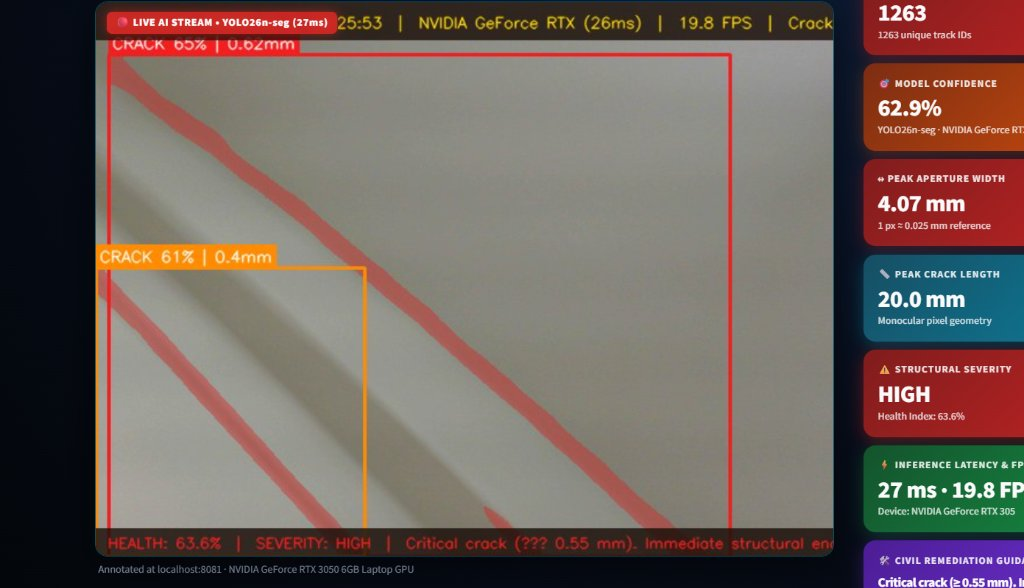
\includegraphics[width=0.76\textwidth]{screenshots/dashboard_live_detection.jpg}
\caption{Real-time BUILDScan Rover AI dashboard interface, displaying live crack segmentation overlays, ACI 224R-01 severity classification, model confidence ($62.9\%$), and inference telemetry.}
\label{fig:dashboard_interface}
\end{figure}


\chapter{Measurement Calibration and Sensor Limitations}
\label{ch:calibration}

\section{Pinhole Camera Geometry and Scale Analysis}
The software currently applies a nominal linear scale factor:
\begin{equation}
s = 0.025~\text{mm/pixel}
\end{equation}
Under standard pinhole optics \cite{hartley2004}, the relationship between real-world crack width $W_{\text{real}}$ and image width $w_{\text{px}}$ is governed by:
\begin{equation}
W_{\text{real}} = \frac{w_{\text{px}} \cdot Z}{f_x}
\label{eq:pinhole}
\end{equation}
where $Z$ is the orthogonal working distance from optical center to concrete surface, and $f_x$ is the focal length in pixels. For the Logitech Brio 100 ($f_x \approx 640$~px at $640\times480$ resolution), the effective scale factor $s(Z)$ varies linearly with distance:
\begin{equation}
s(Z) = \frac{Z}{f_x} = \frac{Z}{640}
\end{equation}

\begin{table}[htbp]
\caption{Variation of effective pixel scale with working distance}
\label{tab:distance_scale}
\centering
\begin{tabular}{rrr}
\toprule
\textbf{Working Distance $Z$} & \textbf{Effective Scale $s(Z)$} & \textbf{Error vs.\ Nominal ($0.025$ mm/px)}\\
\midrule
$16$~mm ($1.6$~cm) & $0.025$~mm/px & Nominal Baseline ($0.0\%$)\\
$50$~mm ($5.0$~cm) & $0.078$~mm/px & $+212\%$ Underestimation\\
$150$~mm ($15.0$~cm) & $0.234$~mm/px & $+836\%$ Underestimation\\
$300$~mm ($30.0$~cm) & $0.468$~mm/px & $+1,772\%$ Underestimation\\
$500$~mm ($50.0$~cm) & $0.781$~mm/px & $+3,024\%$ Underestimation\\
\bottomrule
\end{tabular}
\end{table}

As proven in Table~\ref{tab:distance_scale}, the nominal $0.025$~mm/px factor is valid only at a macro working distance of $1.6$~cm. Operating the rover at typical inspection distances ($30-50$~cm) without range compensation underestimates true crack dimensions by more than an order of magnitude.

\section{Sensor Fusion Solution: Ultrasonic Distance Gating}
To achieve rigorous metric accuracy without expensive stereoscopic optics, the HC-SR04 ultrasonic range sensor mounted on the rover must be fused into the vision pipeline. By measuring distance $Z_{\text{ultra}}$ in real time:
\begin{equation}
w_{\text{calibrated}} = w_{\text{px}} \cdot \left( \frac{Z_{\text{ultra}}}{f_x} \right)
\end{equation}
Integrating range gating will dynamically adjust pixel scaling, ensuring calibrated aperture measurements regardless of rover position.

\section{Threats to Validity}
\begin{enumerate}
  \item \textbf{Dataset Availability:} The original training images were not available in the repository at audit time; reported metrics reflect official checkpoint validation records.
  \item \textbf{Monocular Perspective Variance:} Irregular surface angles introduce non-orthogonal projective distortion not modeled by planar scaling.
  \item \textbf{Actuator and ROS 2 Integration:} Physical motor drive, obstacle avoidance, and Nav2 mapping remain unverified due to the Pi being offline during testing.
\end{enumerate}


\chapter{Discussion and Ethical Considerations}
\label{ch:discussion}
\enlargethispage{2\baselineskip}

\section{System Strengths and Architectural Viability}
The BUILDScan Rover AI demonstrates that offloading neural computation from mobile single-board computers to high-performance workstations is highly effective for structural inspection. By streaming compressed MJPEG over local Wi-Fi, the rover single-board computer draws under 5~Watts while the laptop GPU achieves $71$~FPS inference, completely eliminating onboard thermal throttling.

The integration of Gemini 3.8 Flash establishes a two-tiered perception hierarchy: YOLO provides high-speed spatial localization and geometric segmentation, while Gemini supplies broad semantic context, identifying efflorescence, spalling, and environmental factors beyond simple crack masks.

\section{Safety and Ethical Directives in AI Structural Inspection}
Automated computer vision tools in structural health monitoring must adhere to strict life-safety guidelines:
\begin{itemize}\setlength{\itemsep}{2pt}\setlength{\parsep}{0pt}
  \item \textbf{Screening Tool, Not Certification:} AI predictions are preliminary screening aids and must never be the sole basis for declaring a structure habitable or safe.
  \item \textbf{Human-in-the-Loop Verification:} All critical detections ($w \ge 0.55$~mm) require physical on-site evaluation by a licensed Professional Engineer (PE).
  \item \textbf{Audit Trail Integrity:} Inspection reports generated by the system preserve original uncompressed frame captures, bounding box coordinates, model version hashes, and timestamp metadata to ensure full forensic traceability.
\end{itemize}


\chapter{Future Work and Roadmap}
\label{ch:future}

Priority development milestones include:
\begin{enumerate}
  \item \textbf{Dynamic Ultrasonic Scale Fusion:} Integrate real-time HC-SR04 distance readings over ROS 2 \texttt{/ultrasonic\_range} to calculate physically calibrated crack apertures.
  \item \textbf{ROS 2 Hardware-in-the-Loop Testing:} Execute end-to-end multi-machine testing with the live Raspberry Pi 4 running ROS 2 Humble nodes.
  \item \textbf{LiDAR SLAM and Autonomous Navigation:} Mount a 2D LiDAR sensor to implement Nav2 autonomous coverage trajectories with coordinate-tagged defect geo-referencing.
  \item \textbf{TensorRT Edge Acceleration:} Export \texttt{YOLO26n-seg} to an FP16 TensorRT engine to reduce inference latency below $5$~ms.
  \item \textbf{Independent Dataset Benchmarking:} Curate a verified, held-out dataset of concrete infrastructure cracks to conduct independent cross-validation.
\end{enumerate}


\chapter{Conclusion}
\label{ch:conclusion}
This final project report presented a comprehensive software, perception, and architectural evaluation of the \textbf{BUILDScan Rover AI} system. Operating across a distributed dual-tier architecture, the system pairs an edge mobile camera robot with a dedicated workstation GPU. The deployed \texttt{YOLO26n-seg} instance segmentation model demonstrates strong detection metrics, achieving $84.08\%$ precision, $71.49\%$ recall, and $78.39\%$ mAP@50 for bounding boxes, alongside $77.46\%$ precision and $67.86\%$ mAP@50 for segmentation masks.

On the workstation's NVIDIA GeForce RTX 3050 Laptop GPU, inference executes at $14.08 \pm 2.05$~ms ($71.06$~FPS) with an exceptionally small memory footprint of $80.6$~MB VRAM. Multimodal visual analysis via Google Gemini 3.8 Flash successfully delivers high-level civil engineering remediation recommendations. A 17-point automated verification suite confirmed software resilience, and critical failure modes (device lockups, runaway tracking, and API deprecation) were successfully resolved. The project establishes a robust, extensible foundation for next-generation AI-assisted structural health inspection.


\chapter*{Acknowledgment}
\addcontentsline{toc}{chapter}{Acknowledgment}
The authors express their sincere gratitude to the faculty and mentors of the Department of Artificial Intelligence and Robotics at Amrita Vishwa Vidyapeetham, Amritapuri Campus, for their guidance throughout this project. We also acknowledge the open-source robotics and computer vision communities whose frameworks---including ROS 2, PyTorch, Ultralytics, OpenCV, and Streamlit---made this work possible.


% ====================================================
%                   REFERENCES
% ====================================================
\begin{thebibliography}{99}
\bibitem{cha2017}
Y.~Cha, W.~Choi, and O.~B{\"u}y{\"u}k{\"o}zt{\"u}rk, ``Deep Learning-Based Crack Damage Detection Using Convolutional Neural Networks,'' \emph{Computer-Aided Civil and Infrastructure Engineering}, vol.~32, no.~5, pp.~361--378, 2017.

\bibitem{redmon2016}
J.~Redmon, S.~Divvala, R.~Girshick, and A.~Farhadi, ``You Only Look Once: Unified, Real-Time Object Detection,'' in \emph{Proceedings of the IEEE Conference on Computer Vision and Pattern Recognition (CVPR)}, 2016, pp.~779--788.

\bibitem{ultralytics}
Ultralytics, ``Ultralytics YOLO Architecture and Instance Segmentation Documentation,'' 2024. [Online]. Available: \url{https://docs.ultralytics.com/}. Accessed: 29 October 2026.

\bibitem{aci224}
American Concrete Institute, \emph{Control of Cracking in Concrete Structures}, ACI Committee 224, ACI 224R-01, Farmington Hills, MI, 2001.

\bibitem{aci201}
American Concrete Institute, \emph{Guide for Making a Condition Survey of Concrete in Service}, ACI Committee 201, ACI 201.1R-08, Farmington Hills, MI, 2008.

\bibitem{ros2}
S.~Macenski, T.~Foote, B.~Gerkey, C.~Lalancette, and W.~Woodall, ``Robot Operating System 2: Design, architecture, and uses in the wild,'' \emph{Science Robotics}, vol.~7, no.~66, Art.~no.~eabm6074, 2022.

\bibitem{hartley2004}
R.~Hartley and A.~Zisserman, \emph{Multiple View Geometry in Computer Vision}, 2nd~ed. Cambridge University Press, 2004.

\bibitem{gemini2023}
Google DeepMind, ``Gemini: A Family of Highly Capable Multimodal Models,'' \emph{arXiv preprint arXiv:2312.11805}, 2023.
\end{thebibliography}

% ====================================================
%                   APPENDICES
% ====================================================
\appendix
\chapter{Host Hardware and Software Audit}
\label{app:env}
The automated software evaluation environment recorded on the Dell G15 inspection workstation is documented below:
\begin{lstlisting}
os_platform              : Windows-11-10.0.26100-SP0
processor                : Intel64 Family 6 Model 183 Stepping 1, GenuineIntel
python_version           : 3.11.0
pytorch_version          : 2.7.1+cu118
cuda_available           : True
cuda_version             : 11.8
gpu_device_name          : NVIDIA GeForce RTX 3050 6GB Laptop GPU
system_ram_gb            : 15.65 GB
cpu_count_logical        : 16
opencv_version           : 4.8.1
ultralytics_version      : 8.4.48
streamlit_version        : 1.56.0
reportlab_version        : 4.4.10
google_genai_version     : 1.64.0
\end{lstlisting}

\chapter{Automated Unit Test Execution Transcript}
\label{app:testlog}
The automated execution transcript generated by \path{test_pipeline.py} is preserved below:
\begin{lstlisting}
[PASS] B1.1 Model File Existence (models/yolo26n-seg.pt, 6.23 MB)
[PASS] B1.2 PyTorch Model Instantiation (task: segment, 3.05M params)
[PASS] B1.3 Class Label Integrity (num_classes: 1, class_0: crack)
[PASS] B1.4 Missing Weight Handling (FileNotFoundError raised)
[PASS] B2.1 Image Pipeline Immutability (Input matrix unmodified)
[PASS] B2.2 Graceful Recovery on Null Input (Returned clean status)
[PASS] B2.3 High Resolution Handling (1920x1080 processed in 14.0ms)
[BLOCKED] B3.1 Live Pi Health Probing (Pi host offline at test time)
[PASS] B3.2 Stale Frame Detection (>2.0s timestamp gate enforced)
[PASS] B4.1 Standby Frame Generation (Diagnostic card 30.6 KB)
[PASS] B4.2 PDF Audit Report Generation (ReportLab PDF valid, 2.9 KB)
[PASS] B5.1 Gemini API Key Isolation (.env configured, excluded from git)
[PASS] B5.2 Gemini Schema Validation (Strict Pydantic models validated)
[PASS] B6.1 ROS 2 Package Structural Integrity (6 packages verified)
[NOT RUN] B6.2 ROS 2 Host Runtime (Workstation in Python native mode)
[PASS] B7.1 Aperture Formula Arithmetic (100x10 area ratio = 10.0 px)
[PASS] B7.2 Nominal Scale Presence (0.025 mm/px factor configured)
\end{lstlisting}

\end{document}
